% # COPYRIGHT:
%
% Copyright (C) 2011 Jeremiah Mahler <jmmahler@gmail.com>.
% Permission is granted to copy, distribute and/or modify this document
% under the terms of the GNU Free Documentation License, Version 1.3
% or any later version published by the Free Software Foundation;
% with no Invariant Sections, no Front-Cover Texts, and no Back-Cover Texts.
% A copy of the license is included in the file "fdl-1.3.txt".
%
\documentclass[12pt]{article}
%\usepackage{mslapa}
\usepackage{hyperref}
\usepackage{amsmath}
\usepackage{graphicx}
\usepackage{ulem}
\usepackage{vmargin}
\usepackage{tabularx}
\usepackage{sectsty}
\usepackage{pbox}
\usepackage{bigstrut}
\usepackage{enumerate}
\usepackage{parskip} % add spaces between paragraphs
\input kvmacros % Karnaugh Maps and Veitch charts
%\usepackage{cleveref}
\usepackage{verbatim}

\setpapersize{USletter}
\setmarginsrb{1.0in}{1.0in}{1.0in}{1.0in}{0in}{0.25in}{0in}{0.20in}

\sectionfont{\normalsize}
\subsectionfont{\normalsize}

% configure \bigstrut size
% This configures spacing above and below rows in a tabularx.
%\renewcommand{\bigstrutjot}{6pt}

\renewcommand{\bigstrutjot}{2.0\jot}

\setlength{\parindent}{0in}

\raggedright

\begin{document}

% {{{ Cover Page
\centerline{\bf EECE 144}
\centerline{\bf Fall 2011}
\centerline{\bf}
\centerline{\bf Lab Report \#11}
\centerline{\bf Section 4}
\centerline{\bf 11/16/2011}
% signature area
\begin{center}
\begin{tabularx}{\textwidth}[b]{X l l}
Submitted by: Jeremiah Mahler & & \\
Signature & Printed Name & Date \\
\hline
\multicolumn{1}{|X|}{} & \multicolumn{1}{|l|}{\bigstrut \bf Jeremiah Mahler} & \multicolumn{1}{|l|}{\bf Nov 16, 2011} \\
\hline
\multicolumn{1}{|X|}{} & \multicolumn{1}{|l|}{\bigstrut \bf Marvanee Johnson} & \multicolumn{1}{|l|}{\bf Nov 16, 2011} \\
\hline
\end{tabularx}
\end{center}
% }}}

% {{{ Description/Objectives
\section{Description/Objectives}

The objective of this lab is to design a three bit binary counter
that iterates over the following non-sequential sequence
in ascending order from top to bottom when $X = 0$ and in
descending order when $X = 1$.
The design must use one JK, one T, and one D flip-flop.

\begin{center}
\begin{tabular}[t]{cccc}
0 & 0 & 0 \\
0 & 1 & 0 \\
1 & 1 & 0 \\
0 & 1 & 1 \\
1 & 0 & 1 \\
0 & 0 & 1 \\
1 & 0 & 0 \\
1 & 1 & 1 \\
\end{tabular}
\end{center}

% }}}

% {{{ Procedure
\section{Procedure}
\label{sec:procedure}

To implement this counter one flip flop is used for each bit.
Any type of flip flop can be used for any bit but in this
specific implementation we will use a JK flip-flop for the
most significant bit followed by a T and a D.

The first step is to build a state table which describes all
the required counter states along with the flip-flop inputs
necessary to produce the desired outputs as shown in Table \ref{tbl:st}. 
From this table the mapping from the inputs
($Q_2$, $Q_1$, $Q_0$) to gate inputs ($J_2$, $K_2$, $T_1$, $D_0$) can be determined.

\begin{table}
\center
\begin{tabular}[t]{r|cccc|ccc|cc|c|c}
n & $X$ & $Q_2$ & $Q_1$ & $Q_0$ & $Q_2^+$ & $Q_1^+$ & $Q_0^+$ & $J_2$ & $K_2$ & $T_1$ & $D_0$ \\ 
\hline
0 & 0 & 0 & 0 & 0   & 0 & 1 & 0   & 0 & x   & 1   & 0 \\ 
1 & 0 & 0 & 0 & 1   & 1 & 0 & 0   & 1 & x   & 0   & 0 \\ 
2 & 0 & 0 & 1 & 0   & 1 & 1 & 0   & 1 & x   & 0   & 0 \\ 
3 & 0 & 0 & 1 & 1   & 1 & 0 & 1   & 1 & x   & 1   & 1 \\ 
4 & 0 & 1 & 0 & 0   & 1 & 1 & 1   & x & 0   & 1   & 1 \\ 
5 & 0 & 1 & 0 & 1   & 0 & 0 & 1   & x & 1   & 0   & 1 \\ 
6 & 0 & 1 & 1 & 0   & 0 & 1 & 1   & x & 1   & 0   & 1 \\ 
7 & 0 & 1 & 1 & 1   & 0 & 0 & 0   & x & 1   & 1   & 0 \\ 
8 & 1 & 0 & 0 & 0   & 1 & 1 & 1   & 1 & x   & 1   & 1 \\ 
9 & 1 & 0 & 0 & 1   & 1 & 0 & 1   & 1 & x   & 0   & 1 \\ 
10 & 1 & 0 & 1 & 0   & 0 & 0 & 0   & 0 & x   & 1   & 0 \\ 
11 & 1 & 0 & 1 & 1   & 1 & 1 & 0   & 1 & x   & 0   & 0 \\ 
12 & 1 & 1 & 0 & 0   & 0 & 0 & 1   & x & 1   & 0   & 1 \\ 
13 & 1 & 1 & 0 & 1   & 0 & 1 & 1   & x & 1   & 1   & 1 \\ 
14 & 1 & 1 & 1 & 0   & 0 & 1 & 0   & x & 1   & 0   & 0 \\ 
15 & 1 & 1 & 1 & 1   & 1 & 0 & 0   & x & 0   & 1   & 0 \\ 
\end{tabular}
\caption{State table for  the 3-bit counter using a JK,
T and D flip-flop in order with the JK as the most significant bit.
The "don't care" values are denoted by an x.}
\label{tbl:st}
\end{table}

% {{{ bit $Q_2$ using JK flip-flop
\subsection{bit $Q_2$ using JK flip-flop}

The Karnaugh Maps for bit $Q_2$ are shown in Figure \ref{fig:kmapQ2}.
From this table it can be seen that $J_2$ and $K_2$ are disjoint so
they can be merged in to a single function that represents them both.
This results in the SOP equation shown below.
\begin{align*}
J_2/K_2 &= X' Q_1 + X' Q_0 + Q_2 Q_1 Q_0' + Q_2' Q_0 + X Q_1'
\end{align*}

\begin{figure}
\begin{tabular}{cc}
\karnaughmap{4}{$J_2:$}{{$X$}{$Q_2$}{$Q_1$}{$Q_0$}}{0111XXXX1101XXXX}{}
&
\karnaughmap{4}{$K_2:$}{{$X$}{$Q_2$}{$Q_1$}{$Q_0$}}{XXXX0111XXXX1110}{}
\\
\multicolumn{2}{c}{
\karnaughmap{4}{$J_2/K_2:$}{{$X$}{$Q_2$}{$Q_1$}{$Q_0$}}{0111011111011110}{}
}
\end{tabular}
\caption{Karnaugh Maps for bit $Q_2$ used to describe the mapping from
the inputs ($Q_2$, $Q_1$, $Q_2$, $X$) to the input of the
JK flip-flop ($J_2$, $K_2$).
In this case $J_2$ and $K_2$ are disjoint so they can be merged in
to a single table ($J_2/K_2$).
}
\label{fig:kmapQ2}
\end{figure}
% }}}

% {{{ bit $Q_1$ using T flip-flop
\subsection{bit $Q_1$ using T flip-flop}

The Karnaugh Map for bit $Q_1$ is shown in Figure \ref{fig:kmapQ1}.
This results in the SOP equation shown below.
\begin{align*}
T_1 &= X' Q_1' Q_0' + X' Q_1 Q_0 + X Q_2 Q_0 + X Q_2' Q_0'
\end{align*}

\begin{figure}
\center
\karnaughmap{4}{$T_1:$}{{$X$}{$Q_2$}{$Q_1$}{$Q_0$}}{1001100110100101}{}
\caption{Karnaugh Map for bit $Q_1$ used to describe the mapping from
the inputs ($Q_2$, $Q_1$, $Q_2$, $X$) to the input of the T flip-flop $T_1$.}
\label{fig:kmapQ1}
\end{figure}
% }}}

% {{{ bit $Q_0$ using D flip-flop
\subsection{bit $Q_0$ using D flip-flop}

The Karnaugh Map for bit $Q_0$ is shown in Figure \ref{fig:kmapQ0}.
This results in the SOP equation shown below.
\begin{align*}
D_0 &= Q_2 Q_1' + X' Q_2 Q_0' + X Q_1' + X' Q_2' Q_1 Q_0
\end{align*}

\begin{figure}
\center
\karnaughmap{4}{$D_0:$}{{$X$}{$Q_2$}{$Q_1$}{$Q_0$}}{0001111011001100}{}
\caption{Karnaugh Map for bit $Q_0$ used to describe the mapping from
the inputs ($Q_2$, $Q_1$, $Q_2$, $X$) to the input of the D flip-flop $D_0$.}
\label{fig:kmapQ0}
\end{figure}
% }}}

% {{{ circuit construction
\subsection{circuit construction}

After all the equations for each bit has been found these
can be combined together to produce a complete solution that works
for all bits and implements the 3-bit, non-sequential counter.
In this case Logisim\cite{LOGISIM} will be used to build and simulate the circuit.

This implementation has many interconnections so its construction
can be quite tedious.
The resulting circuit is shown in Figure \ref{fig:circ}.
Every single combination should be verified against the
state table (Table \ref{tbl:st}) to ensure every connection is right.

In the event of an error it is best to methodically diagnose the error
rather than removing all or some and starting over.
Starting over does nothing to find the problem and it is possible that
the problem could be built again if the design is wrong.
A good strategy for finding problems is to try and isolate the problem.
For example, if the bit $Q_2$ is wrong it would make sense to check
the JK flip-flop since that is the bit it controls.

\begin{figure}
\center
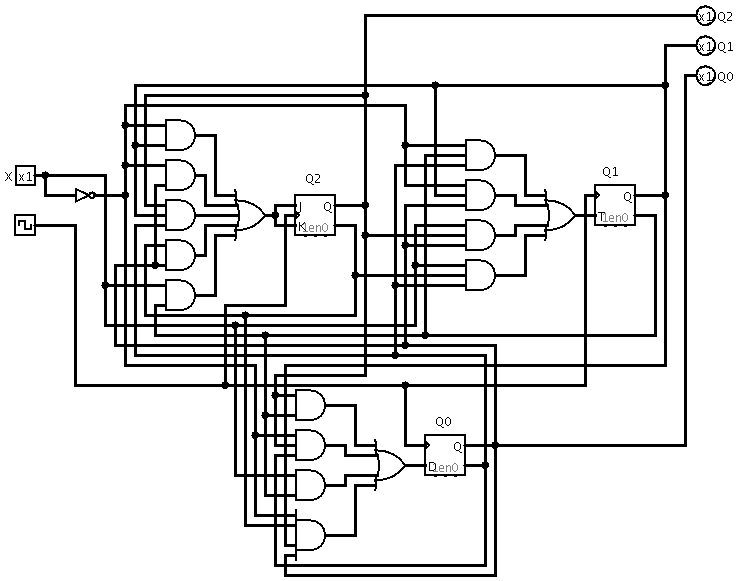
\includegraphics[scale=0.5]{lab11-circuit}
\caption{Circuit diagram of 3 bit-counter.}
\label{fig:circ}
\end{figure}

% }}}

% }}}

% {{{ Observations
\section{Observations}

\samepage
The counter, when simulated in Logisim, reproduced the desired sequence
in both the up and down directions.

Due to the tedious nature of this design several errors did
occur while building the circuit which had to be fixed.
The strategy of trying to isolate the problem to a specific bit
or part of the circuit worked well.

The complexity of this design suggests that there may be a simpler
solution.
One possible avenue for optimization is the input gates to the flip-flops.
Perhaps these can be aggregated together to use fewer gates.
Another possibility is to try different gate types in different positions.
Perhaps a JK would require fewer gates as bit 1 instead of bit 2 for example.

% }}}

% {{{ Conclusion
\section{Conclusion}

This lab was a success in designing and implementing a
three bit non-sequential up/down counter in Logisim
using three flip-flops of different types.
It is indeed possible to build a counter with three different
types of flip-flops along with several additional gates.

% }}}

%\clearpage

\renewcommand*{\refname}{\vspace{-8mm}}
\section{References}
%%\bibliographystyle{plain}
%%\bibliographystyle{mslapa}
\bibliographystyle{ieeetr}
\bibliography{../references}

\end{document}

% vim:foldmethod=marker
